\documentclass{standalone}

\usepackage{tikzlings}

\begin{document}

\begin{tabular}{ccccccccccccc}

\begin{tikzpicture}
	\bear
\end{tikzpicture}	
&

\begin{tikzpicture}
	\penguin
\end{tikzpicture}	
&

\begin{tikzpicture}
	\marmot
\end{tikzpicture}	
&

\begin{tikzpicture}
	\koala
\end{tikzpicture}	
&

\begin{tikzpicture}
	\owl
\end{tikzpicture}	
&

\begin{tikzpicture}
	\coati
\end{tikzpicture}	
&

\begin{tikzpicture}
	\snowman
\end{tikzpicture}	
&

\begin{tikzpicture}
	\mouse
\end{tikzpicture}	
&

\begin{tikzpicture}
	\moles
\end{tikzpicture}	
&

\begin{tikzpicture}
	\sloth
\end{tikzpicture}	
&

\begin{tikzpicture}
	\cat
\end{tikzpicture}	
&

\begin{tikzpicture}
	\pig
\end{tikzpicture}	
&

\begin{tikzpicture}
	\hippo
\end{tikzpicture}	
\\

\begin{tikzpicture}
	\bear[3D]
\end{tikzpicture}	
&

\begin{tikzpicture}
	\penguin[3D]
\end{tikzpicture}	
&

\begin{tikzpicture}
	\marmot[3D]
\end{tikzpicture}	
&

\begin{tikzpicture}
	\koala[3D]
\end{tikzpicture}	
&

\begin{tikzpicture}
	\owl[3D]
\end{tikzpicture}	
&

\begin{tikzpicture}
	\coati[3D]
\end{tikzpicture}	
&

\begin{tikzpicture}
	\snowman[3D]
\end{tikzpicture}	
&

\begin{tikzpicture}
	\mouse[3D]
\end{tikzpicture}	
&
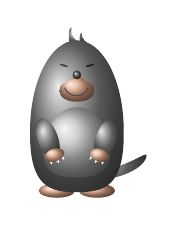
\begin{tikzpicture}
	\moles[3D]
\end{tikzpicture}	
&

\begin{tikzpicture}
	\sloth[3D]
\end{tikzpicture}	
&

\begin{tikzpicture}
	\cat[3D]
\end{tikzpicture}	
&

\begin{tikzpicture}
	\pig[3D]
\end{tikzpicture}	
&

\begin{tikzpicture}
	\hippo[3D]
\end{tikzpicture}	
\end{tabular}

\end{document}
